\chapter{Link}
\href{https://sites.google.com/site/compilerclassunitn/}{Vecchio sito}\\
\href{https://docs.google.com/document/d/12NLo0B3TjlFMs4CbMqYd3q64-wBdG0KhpjzqsvZ5wrI/edit}{Note Drive}\\

%%%%%%%%%%%%%%%%%%%%%%%%%%%%%%%%%%%%%%%%%%%%%%%%%%%%%%%%%%%%%%%%%%%%%%%%%%%%%%%%%%%%%%%%%%%%%%%%%%%%%%%%%%%
\chapter{Introduzione}

I linguaggi di \textbf{analisi lessicale} lavorano con simboli e caratteri; devo costruire una \textbf{tavola dei simboli} (specifica per un dato programma e compilatore). L'analisi restituisce dei \textbf{tokens} (puntatori) a record nella tavola dei simboli.
La maggior parte delle implementazioni usano un numero come \textbf{identificatore}.

\textbf{L'analisi sintattica} invece studia la \textbf{grammatica del linguaggio}. Viene costruito un \textbf{abstract syntax tree}:

\begin{center}
	$a = b + c \cdot 60$
\end{center}

\Tree [.= $a$ [.+ $b$ [.* $c$ $60$ ] ] ]
\Tree [.assegnamento $id_1$ [.+ $id_2$ [.* $id_3$ $id_4$ ] ] ]

\textbf{L'analisi semantica} si occupa di vedere se c'\'e una corretta semantica (variabili dichiarate precedentemente). 
Se * necessita di un float allora 60 dev'essere convertito a float. 

\begin{center}
	\Tree [.* {\ldots} [.{intToReal(num)} 60.0 ] ]\\[5pt]
\end{center}

Generazione di \textbf{codice intermedio}: 
\begin{tabular}{ll|l}
$temp_1$ =& intToReal(60) & \\
$temp_2$ =& $id_3 * temp1$ & VISITA DELL'ALBERO\\
$temp_3$ =& $id_2 + temp2$ & \\
$id_1$ =& $temp_3$ & \\
\end{tabular}\\[5pt]

\Tree [.D [.\fbox{Codice intermedio} $M1$ $M2$ $M3$ ] ]\\[5pt]

%%%%%%%%%%%%%%%%%%%%%%%%%%%%%%%%%%%%%%%%%%%%%%%%%%%%%%%%%%%%%%%%%%%%%%%%%%%%%%%%%%%%%%%%%%%%%%%%%%%%%%%
\section{Grammatiche}

Una \textbf{grammatica} \'e una tupla G(V, T, S, P) con:
\begin{tabular}{ll}
V & vocabolario\\
T & set simboli terminali\\
S & start symbol\\
P & set delle produzioni\\
V$\backslash$T & simboli\\
$\varepsilon$ & parola vuota, non pu\'o essere un terminale!\\
%[Sono tutti insiemi!] & \\
\end{tabular}\\[5pt]

Le produzioni sono della forma $\alpha \rightarrow \beta$ con $\alpha$ 
\textbf{stringa non vuota di simboli V con almeno un non terminale},
$\beta $ stringa su V o $\varepsilon $.


\begin{tcolorbox}\begin{center}
Per convenzione i caratteri in maiuscolo denotano simboli non terminali mentre in minuscolo terminali. Quindi i simboli in T sono 
tutti lettere minuscole.
\end{center}\end{tcolorbox}

Considero X, Y variabili, generico simbolo in V e $\alpha\ \beta\ \delta\ \text{stringhe su } V^*$ \\
\begin{tabular}{l}
$S \rightarrow aSb$ \\
$S\rightarrow \varepsilon$\\
$S \rightarrow A$\\
\end{tabular}
$T=\{a, b\}$ (terminali), ($V\backslash T) = \{S, A\} $ (non terminali)\\

%%%%%%%%%%%%%%%%%%%%%%%%%%%%%%%%%%%%%%%%%%%%%%%%%%%%%%%%%%%%%%%%%%%%%%%%%%%%%%%%%%%%%%%%%%%%%%%%%%%%%%%%%%%
\subsection{Derivazioni}
Date 
$\mu = \mu_1 \alpha \mu2,\ \alpha \rightarrow \beta$, produzioni della grammatica G, $\gamma = \mu_1 \beta \mu_2$ \'e una 
derivazione in uno o pi\'u passi partendo da $\mu$.\\

Scrivendo $\mu \rightarrow ^+ \gamma $ intendo che posso derivare $\gamma$ da $\mu$ in uno o pi\'u passi di derivazione.

%%%%%%%%%%%%%%%%%%%%%%%%%%%%%%%%%%%%%%%%%%%%%%%%%%%%%%%%%%%%%%%%%%%%%%%%%%%%%%%%%%%%%%%%%%%%%%%%%%%%%%%%%%%
\subsection{Linguaggio generato da una grammatica}
\begin{center}
	$L(G) = \{w\ / \ w \in T^*, S \rightarrow ^{+}_{G} w \} $
\end{center}
Dato il linguaggio L possono esistere pi\'u grammatiche diverse tra loro che generano L.
Pertanto dal linguaggio non posso risalire con certezza alla grammatica.

\begin{tcolorbox}\begin{center}
	In generale dato un linguaggio generale L ed una grammatica G $\not\exists$ un algoritmo per dimostrare che L = L(G).
\end{center}\end{tcolorbox}

%%%%%%%%%%%%%%%%%%%%%%%%%%%%%%%%%%%%%%%%%%%%%%%%%%%%%%%%%%%%%%%%%%%%%%%%%%%%%%%%%%%%%%%%%%%%%%%%%%%%%%%%%%%
\chapter{Linguaggi liberi}
\section{Grammatica libera dal contesto (context free)}
Una grammatica generata \'e libera dal contesto (context free) se ogni sua produzione ha la forma: 

\begin{center}
	$A \rightarrow \beta$
\end{center}
Con A non terminale. ($\alpha \rightarrow \beta$, $\alpha$ deve essere un solo simbolo non terminale, altrimenti \'e condizionata).\\
Con $\beta$ qualsiasi (terminali, non terminali o $\varepsilon$).\\[5pt]
Grammatiche libere si prestano in modo naturale a descrivere derivazioni in viste ad albero.

%%%%%%%%%%%%%%%%%%%%%%%%%%%%%%%%%%%%%%%%%%%%%%%%%%%%%%%%%%%%%%%%%%%%%%%%%%%%%%%%%%%%%%%%%%%%%%%%%%%%%%%%%%%
\subsection{Esempi}
\begin{tabular}{l}
	$S \rightarrow aAb$\\
	$aA \rightarrow aaAb$\\
	$A \rightarrow \varepsilon$\\
\end{tabular}
Non \'e context free, genera $L(G) = \{ a^nb^n\ / \ n>0 \}$.\\[5pt]
%%
\begin{tabular}{l}
	$S \rightarrow aSb | \varepsilon$\\
	$S \rightarrow aSb \rightarrow aaSbb \rightarrow aabb \implies \{a^nb^n\ / \ n \geq 0 \} $ \\
\end{tabular}
Context free, genera lo stesso L di quella sopra.\\
Serve per parentesizzare correttamente codice (genera $a^n b^n$).\\[5pt]
%%
\begin{tabular}{l}
$S \rightarrow AB$\\
$A \rightarrow Aa|a$\\
$B \rightarrow Bb|b$\\
\end{tabular}
Tutto ci\'o che deriva da A \'e indipendente da ci\'o che deriva da B. ${a^{n}b^{m},\ n, m \geq 0}$\\[5pt]
%%
Se ho produzioni impossibili che non finiscono in terminali la grammatica genera un linguaggio vuoto (
$(\{ S, B, a \},\ \{ A \} ,\ S,\ \{ S\rightarrow aB \})$).\\[5pt]
%%
$(\{ S\} ,\ \{ \},\ S,\ \{ S \rightarrow \varepsilon \} )$ invece genera un linguaggio $\{ \varepsilon \} \not = \emptyset $\\[5pt]
%%
\begin{tabular}{l}
$S \rightarrow 0B | 1A$\\
$A \rightarrow 0|0S|1AA$\\
$B \rightarrow 1|1S|0BB$\\
\end{tabular}
L(G) = \{w \ / \ count(0,w)=count(1,w) \}\\[5pt]
%%
Definire una grammatica per $L = (a^kb^n \ / \ k, n > 0)$\\
\begin{tabular}{l}
	$S \rightarrow aS|aB$\\
	$B \rightarrow bB|b$\\
\end{tabular}
\begin{tabular}{l}
	$S\rightarrow AB$\\
	$A \rightarrow aA|a$\\
	$B \rightarrow bB|b$\\
\end{tabular}
\begin{tabular}{l}
	$S \rightarrow ab|aS|Sb$\\
\end{tabular}\\[5pt]
%%
Definire G tale che $L(G) = \{ a^kb^nc^{2n} \ / \ k,n >0 \}$
\begin{tabular}{l}
	$ S \rightarrow AB$\\
	$ A \rightarrow aA|a$\\
	$ B \rightarrow bBcc|bcc$\\
\end{tabular}\\[5pt]
%%
Definire G tale che $L(G) = \{ a^kb^nd^{2k} \ / \ k, n >0 \}$
\begin{tabular}{l}
	$S \rightarrow aSdd | B$\\
	$B \rightarrow bB|b$\\
\end{tabular}\\[5pt]
\begin{tabular}{l}
	$S \rightarrow aSdd|aBdd$\\
	$B \rightarrow bB|b$\\
\end{tabular}\\[5pt]

%%%%%%%%%%%%%%%%%%%%%%%%%%%%%%%%%%%%%%%%%%%%%%%%%%%%%%%%%%%%%%%%%%%%%%%%%%%%%%%%%%%%%%%%%%%%%%%%%%%%%%%%%%%
\section{Abstract syntax Tree}
\begin{center}
$S \rightarrow aSb|ab$
\end{center}
\Tree [.S a [.S a b ] b ] 

aabb, derivazione canonica $\mu \rightarrow \gamma$

%%%%%%%%%%%%%%%%%%%%%%%%%%%%%%%%%%%%%%%%%%%%%%%%%%%%%%%%%%%%%%%%%%%%%%%%%%%%%%%%%%%%%%%%%%%%%%%%%%%%%%%%%%%
\section{Grammatiche ambigue}
Nel caso di grammatiche libere si definiscono le \textbf{derivazioni canoniche destre e sinistre}, nel caso \textbf{rightmost} si richiede che ad ogni passo di derivazione $\mu \rightarrow \gamma $ venga rimpiazzato il terminale pi\'u a destra di $\mu $; nel caso 
\textbf{leftmost} quello pi\'u a sinistra.\\
\begin{tcolorbox}\begin{center}
	G \'e \textbf{ambigua} se esiste una parola del linguaggio generato da G, generabile con due derivazioni canoniche distinte entrambe destre o entrambe sinistre.
\end{center}\end{tcolorbox}

$E \rightarrow E+E|E*E|4$ (il + associa a sinistra)
\begin{center}
	\Tree[.E [.E [.E 4 ] + [.E 4 ] ] + [.E 4 ] ]
	\Tree[.E [.E 4 ] + [.E [.E 4 ] + [.E 4 ] ] ]
\end{center}
\begin{center}
	\Tree[.+ [.+ 4 4 ] 4 ]
	\Tree[.+ 4 [.+ 4 4 ] ]
\end{center}
[Analogo con il *] Essendo derivazioni entrambe leftmost \textbf{G \'e ambigua}.\\

\begin{tcolorbox}\begin{center}
	Occhio a non confondere la struttura dell'albero di derivazione con la sua sequenza di derivazioni.\\
	La derivazione leftmost sostituisce prima i non terminali a sinistra e poi procede con i successivi.\\
	Quello a sx prima spacca la E in E+E che poi viene spaccato in E+E dove poi vanno sostituiti alle E i non terminali 4.\\
	Quello a dx invece spacca E in E+E, sostituisce alla prima E il 4 e poi passa alla sostituzione della seconda E con E+E.\\
	In entrambi i casi la sostituzione dei non terminali avviene sempre prendendo il primo non terminale della stringa, cio\'e quello pi\'u a sinistra.\\[5pt]

	Finch\'e considero sostituzioni con un solo carattere a destra della produzione leftmost e rightmost sono del tutto equivalenti; 
	la differenza arriva quando considero produzioni con sostituzioni su pi\'u di un carattere perch\'e mangi caratteri a possibili derivazioni future.
\end{center}\end{tcolorbox}

\begin{tabular}{l}
$S \rightarrow if\ b\ then\ S\ |\ if\ b\ then\ S\ else\ S\ |\ altro$\\
$if\ b\ then\ if\ b\ then\ altro\ else\ altro$\\
$if\ b\ then\ S\ else\ S$\\
\end{tabular}\\

%%%%%%%%%%%%%%%%%%%%%%%%%%%%%%%%%%%%%%%%%%%%%%%%%%%%%%%%%%%%%%%%%%%%%%%%%%%%%%%%%%%%%%%%%%%%%
\section{Linguaggi liberi}
\begin{tcolorbox}\begin{center}
	Un linguaggio \'e libero se esiste una grammatica libera che lo genera. 
\end{center}\end{tcolorbox}

\textbf{Lemma 1}: La classe dei linguaggi liberi \'e \textbf{chiusa all'unione} 
(se $L_1$ e $L_2$ sono liberi allora $L1 \cup L2$ \'e ancora libero)
\begin{equation}\begin{split}
	L_1\ libero\ & \implies \exists G_1=(V_1,T_1,S_1,P_1)\ / \ L_1 = L(G_1)\\
	L_2\ libero\ & \implies \exists G_2=(V_2,T_2,S_2,P_2)\ / \ L_2 = L(G_2)\\
	(\{ V_1 \cup V_2 \cup \{ S \},T_1 \cup T_2, & S,P_1 \cup P_2 \cup (S \rightarrow S_1|S_2) \})\\
\end{split}\end{equation} 

Devo rinominare i non terminali di G1 e G2 in modo da non avere omonimie (clash). 
Notare la produzione che agginge un nuovo start symbol per agganciarsi ai vecchi.\\[5pt]

\textbf{Lemma 2}: La classe dei linguaggi liberi \'e \textbf{chiusa rispetto alla concatenazione}
(se L1 e L2 sono liberi allora 
$\{w_1w_2 \ / \ w_1 \in L_1,\ w_2 \in L_2 \}$ \'e esso stesso un linguaggio libero).
\begin{center}
	$G = (V_1 \cup V'_2 \cup \{ S \},\ T_1 \cup T_2,\ S,\ P_1 \cup P'_2 \cup \{ S \rightarrow S_1S'_2\} )$
\end{center}

$P_1 \cup P_2 \cup \{ S \rightarrow S_1 S_2 \}$ anche in questo caso bisogna stare attenti ad eliminare possibili clash dei simboli non terminali di $G_2$. Metto un apice per indicare una rinominazione dei non terminali ($V'_2,\ S'_2,\ P'_2$). In pratica concateno gli start symbols.

%%%%%%%%%%%%%%%%%%%%%%%%%%%%%%%%%%%%%%%%%%%%%%%%%%%%%%%%%%%%%%%%%%%%%%%%%%%%%%%%%%%%%%%%%%%%%%%%
\subsection{Esempio}
Il linguaggio $\{ a^nb^n\ / \ n > 0 \}$ \'e libero perch\'e $\exists$ una grammatica libera che lo genera ($G_1$):\\
\begin{center}
	$G_1\qquad S\rightarrow aSb/ab$ $G_1$ libera\\
	$G_2\qquad s\rightarrow aAb,\ A\rightarrow aaAb,\ A\rightarrow \varepsilon$ $G_2$ non libera $\Box$\\
\end{center}   

%%%%%%%%%%%%%%%%%%%%%%%%%%%%%%%%%%%%%%%%%%%%%%%%%%%%%%%%%%%%%%%%%%%%%%%%%%%%%%%%%%%%%%%%%%%%%%%%
\section{Pumping Lemma per Linguaggi Liberi}
\begin{tcolorbox}\begin{center}
	Serve per dimostrare che un linguaggio non \'e libero. Ossia non esiste alcuna grammatica libera che lo genera.
\end{center}\end{tcolorbox}

\textbf{Pumping lemma}: 

Sia L un linguaggio libero allora $\exists p \in \mathbb{N}^+ \ / \ \forall z \in L \ / \ |z| > p,\exists u v w x y:$
\begin{itemize}
	\item[i)] 	$z = uvwxy\ \land$ \\
	\item[ii)] 	$|vwx| \geq p\ \land$ \\
	\item[iii)] $|vx| > 0 \ \land$ \\
	\item[ ] 	$\forall i \in \mathbb{N} \ / \ uv^iwx^iy \in L$\\
\end{itemize}

%%%%%%%%%%%%%%%%%%%%%%%%%%%%%%%%%%%%%%%%%%%%%%%%%%%%%%%%%%%%%%%%%%%%%%%%%%%%%%%%%%%%%%%%%%%%
\subsection{Commento definizione}
\begin{tabular}{ll}
$\exists\ p\in \mathbb{N}^+$ & esiste una costante $p>0$\\
$\forall\ z\in L:\ |z|>p$ & ogni parola con pi\'u elementi di p\\
$\exists\ uvwxy \ / \ z = uvwxy $ & esistono 5 sottostringhe che compongono z\\
$|vwx| \leq p$ & la lunghezza delle 3 stringhe centrali \'e minore di p\\
$|vx|>0$ & la seconda e la quarta non sono mai entrambe nulle\\
$\forall\ i \in \mathbb{N} uv^iwx^iy \in L$ & se ripeto i volte (i pu\'o essere 0) la 2 e la 4 sono ancora in L\\
\end{tabular}

%%%%%%%%%%%%%%%%%%%%%%%%%%%%%%%%%%%%%%%%%%%%%%%%%%%%%%%%%%%%%%%%%%%%%%%%%%%%%%%%%%%%%%%%%%%%%%
\subsection{Dimostrazione Pumping Lemma}
\textbf{Osservazione 1}:
Data una grammatica G posso sempre creare una altra grammatica G' modificata dalla prima che genera lo stesso linguaggio.\\[5pt]

\textbf{Osservazione 2}:
Una grammatica si pu\'o portare in forma normale (di Chomsky) togliendo eventuali ridondanze o produzioni che terminano per forza con 
$\varepsilon $ (a meno che non debba fare parte del linguaggio, ma a quel punto si scrive come $S \rightarrow \varepsilon$).\\[5pt]

%%%%%%%%%%%%%%%%%%%%%%%%%%%%%%%%%%%%%%%%%%%%%%%%%%%%%%%%%%%%%%%%%%%%%%%%%%%%%%%%%%%%%%%%%%%%%%
\subsubsection{CNF}
Chomsky Normal Form esige che una grammatica non abbia produzioni ridondanti:\\
ie) $\qquad G_1 \qquad S \rightarrow aSb|ab|B,\ B\rightarrow aBb|ab \leftarrow$ doppioni\\

\textbf{Dimostrazione}:
L \'e un linguaggio libero $\implies \exists\ G $ in Chomsky Normal Form tale che L = L(G).\\

Definisco p come la lunghezza della parola pi\'u lunga che pu\'o essere derivata usando un albero di derivazione i cui cammini dalla radice sono lunghi 
al pi\'u come il numero di simboli terminali della grammatica ($|V\backslash T|$).

$S \rightarrow aSb | ab$, ha due terminali, p = 2 
\begin{center}
	\Tree[.S a b ]
	\Tree[.S a [.S a b ] b ]
	\Tree[.S a [.S a [.S a b ] b ] b ]
\end{center}

Guardo il cammino S $\rightarrow S_1 \rightarrow S_2 \rightarrow ... \rightarrow S_K$ di lunghezza K
Se $z \in L\ \land \ |z| > p \implies $ nell'albero di derivazione di z esiste almeno un cammino la cui lunghezza \'e maggiore di 
$|V\backslash T|\implies $ allora esiste almeno un non-terminale che occorre almeno due volte lungo quel cammino (S, nell’esempio sotto).

\begin{center}
	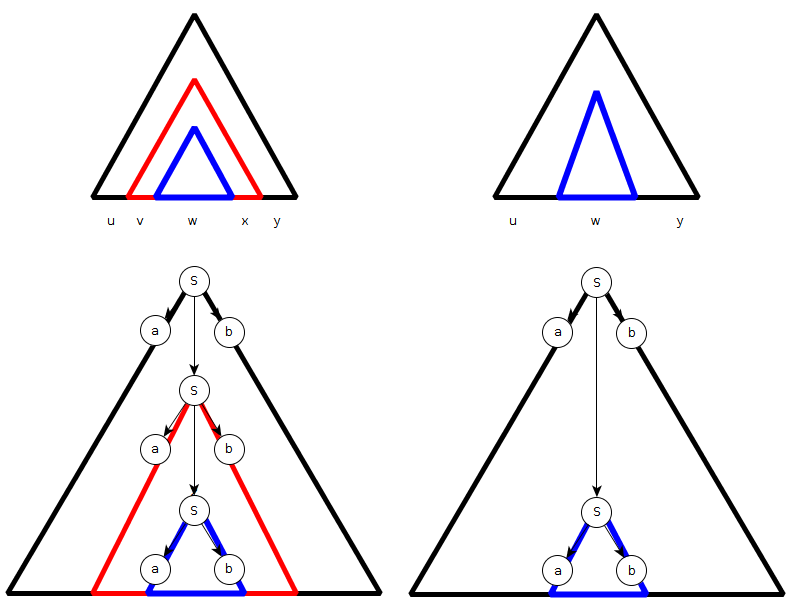
\includegraphics[scale=0.4]{Chapters/Img/c01_05.png}\\
\end{center}

ie) p = 2, se prendo una qualunque parola pi\'u lunga di 3 generata da G: aaaabbbb, la posso dividere in 5 con due pumpable:
u=aa, v=a, w=abb, x=b, y=b 

Se prendo $z\in L \land |z| > p \implies $ ho dovuto usare un albero di derivazione $\ / \ \exists $ al meno un cammino pi\'u lungo 
di $|V\backslash T|$ per definizione di z.
$\implies $ ho un non terminale ripetuto al meno due volte 
$\implies \exists$ al meno un non terminale che occorre al meno 2 volte lungo quel cammino

con \textbf{l'un-pumping} la parola sta sempre nel linguaggio (\textbf{taglio un pezzo di albero}) 
Dato che w e x non possono essere entrambi nulli al massimo avr\'o  $A \rightarrow aA,\ o\ A \rightarrow Aa$

\begin{center}
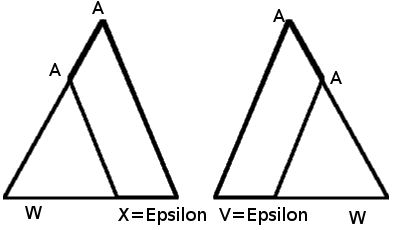
\includegraphics[scale=0.4]{Chapters/Img/c01_03.png}
\end{center}

ie) linguaggio libero $\{a,b\},\ S \rightarrow ab$ 
\begin{center}
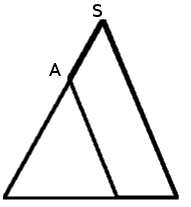
\includegraphics[scale=0.4]{Chapters/Img/c01_04.png}
\end{center}

%%%%%%%%%%%%%%%%%%%%%%%%%%%%%%%%%%%%%%%%%%%%%%%%%%%%%%%%%%%%%%%%%%%%%%%%%%%%%%%%%%%%%%%%%%%%%

\section{Pumping Lemma per assurdo}
(tesi) = L libero $ \implies \exists p \in \mathbb{N}^+ \ / \ \forall z \in L \ / \ |z| > p,\exists u v w x y:$
\begin{itemize}
	\item[i)] 	$z = uvwxy\ \land$ \\
	\item[ii)] 	$|vwx| \geq p\ \land$ \\
	\item[iii)] $|vx| > 0 \ \land$ \\
	\item[ ] 	$\forall i \in \mathbb{N} \ / \ uv^iwx^iy \in L$\\
\end{itemize}
$\neg (tesi) = \forall p \in \mathbb{N}^+ \ / \ \exists z \in L \ / \ |z| > p\ \forall\ uvwxy \ / \ $
$[(z = uvwxy \land |vwx| \leq p \land |vx| > 0)$\\
$\implies \exists i \in N \ / \ uv^iwx^iy \not\in L]$\\[5pt]
%%
\begin{tcolorbox}\begin{center}
	Se si verifica la tesi negata il linguaggio non \'e libero.\\
\end{center}\end{tcolorbox}
%%
Suppongo $L_1 = { w_1 w_2 \ / \ w_1 = w_2,\ w_1, w_2 \in \{a, b\}^*}$ \textbf{libero};\\
Sia p un naturale qualunque sempre positivo;\\
Sia $z = a^p b^p a^p b^p$ ($|z| = 4p$);\\
Allora $z \in L_1,\ |z| > p$\\
Siano $uvwxy \ / \ z=uvwxy,\ |vwx| \leq p \land |vx| > 0$ distinguiamo vari casi:

\begin{itemize}
\item[1)] vwx \'e composto da \lq a\rq\ che occorrono a sinistra ($w_1$)\\
\item[2)] vwx \'e a cavallo e contiene sia \lq a\rq\ che \lq b\rq\ in $w_1$\\
\item[3)] vwx contiene solo \lq b\rq\ in $w_1$\\
\item[4)] \lq b\rq\ in $w_1$ e \lq a\rq $\in w_2$\\
\item[5,6,7)] ...speculare su $w_2$\\
\end{itemize} 
\begin{itemize}
	\item Nei casi 1, 3, 5, 7 considero le parole $z^1=uv^0wx^0y$ (i=0);\\
	\item[-] nel caso 1 sono certo di togliere alcune occorrenze di a quindi avr\'o $z^1 = a^k b^p a^p b^p,\ k < p \implies z^1 \not\in L$. \\
	\item[-] Nel caso 3 $z^1 = a^p b^k a^p b^p,\ k < p \implies z^1 \not\in L$.\\
	\item[-] Nel caso 5 $z^1 = a^p b^p a^k b^p,\ k < p \implies z^1 \not\in L$.\\
	\item[-] Nel caso 7 $z^1 = a^p b^p a^p b^k,\ k < p \implies z^1 \not\in L$.\\
	\item Nei casi 2, 4, 6 invece avr\'o ancora $ z^1=uv^0wx^0y $ (i=0);\\
	\item[-] Nel caso 2 $z^1 = a^k b^p a^p b^p,\ o\ a^p b^k a^p b^p,\ o\ a^j b^k a^p b^p,\ j,k < p \implies z^1 \not\in L$ .\\
	\item[-] ...\\
\end{itemize}
In pratica facendo l'unpumping in tutti i casi $z_1 \not\in L$ quindi L non \'e libero.

%%%%%%%%%%%%%%%%%%%%%%%%%%%%%%%%%%%%%%%%%%%%%%%%%%%%%%%%%%%%%%%%%%%%%%%%%%%%%%%%%%%%%%%%%%%%%%%%%%%%%%%%%%%%%%%%%%%%%%%%%%%%%%%%%%%%%%%%%%%%%%%%%%%%%%%%%%%%%%%%
\subsection{How not to use Pumping Lemma}
Se avessi preso $\{ww \ / \ w\in\{a,b\}^*\}$ sia $z = (ab)^p (ab)^p$, prendo p=4, $v\in\varepsilon, x=a, i = 0$ cos\'i non 
dimostro niente perch\'e se voglio dimostrare con il pumping lemma la negazione della tesi devo dimostrare un asserto che vale $\forall p \in \mathbb{N}^+$.
Pertanto non posso prendere un arbitrario p=4.


%%%%%%%%%%%%%%%%%%%%%%%%%%%%%%%%%%%%%%%%%%%%%%%%%%%%%%%%%%%%%%%%%%%%%%%%%%%%%%%%%%%%%%%%%%%%%%%%%%%%%%%%%%%%%%%%%%%%%%%%%%%%%%%%%%%%%%%%%%%%%%%%%%%%%%%%%%%%%%%%
\subsection{Esempi}
ie) $\{a^nb^nc^j/n,j\geq 0\}=L_{17}$\\
$S \rightarrow aSb|B$\\
$B \rightarrow cB|\varepsilon $\\
$acb \in L_{17}$\\
\begin{center}
	\Tree[.S a b [.S a b [.S $\varepsilon$ ] ] ]
	\Tree[.S a [.S [.B c [.B $\varepsilon$ ] ] ] b ]
\end{center}

$S \rightarrow abA|B$\\
$B \rightarrow cB|\varepsilon$\\s
\begin{center}
	\Tree[.S [.A ... ... ] [B ... ... ] ]\\
\end{center}

$S \rightarrow AB$\\
$A \rightarrow aAb|ab|\varepsilon$\\
$B \rightarrow Ab|c|\varepsilon$\\
\begin{center}
	\Tree[.S [.A a [.A $\varepsilon$ ] b ] [.B $\varepsilon$ ] ]
	\Tree[.S [.A a b ] [.B $\varepsilon$ ] ]
\end{center}

%%%%%%%%%%%%%%%%%%%%%%%%%%%%%%%%%%%%%%%%%%%%%%%%%%%%%%%%%%%%%%%%%%%%%%%%%%%%%%%%%%%%%%%%%%%%%%%%%%%%%%%%%%%%%%%%%%%%%%%%%%%%%%%%%%%%%%%%%%%%%%%%%%%%%%%%%%%%%%%%
\subsection{Esempi Linguaggi Liberi}
Essendo un linguaggio libero chiuso rispetto alla concatenazione, dati:\\

$L_1 = \{a^nb^nc^j \ / \ n, j \geq 0\} $ Libero perch\'e concatenazione di $\{a^nb^n\ / \ n \geq 0 \}$ e $\{ c^j \ / \ j \geq 0 \}$, entrambi liberi\\
$L_2 = \{a^jb^nc^n \ / \ n,j \geq 0\}$ Libero, inverso di $L_1$\\
$L_3 = \{a^nb^nc^n \ / \ n \geq 0\}$ Non \'e libero:

Suppongo $L_3$ libero, sia $p \in \mathbb{N}^+$, $z = a^pb^pc^p$
Allora $z \in  L_3,\ |z|=3p>p$\\
Spacco z in $A=a...a,\ B = b...b, C=c...c$\\
Siano $z = uvwxy\ \land\ |vwx| \leq p \ \land\ |vx| > 0 $:
\begin{itemize}
    \item vwx \'e composto da sole a in A\\
    \item vwx \'e composto da a in A e b in B\\
    \item vwx \'e composto da sole b in B\\
    \item vwx \'e composto da b in B e c in C\\
    \item vwx \'e composto da sole c in C\\
\end{itemize} 
Considero la parola $z' = uv^0wx^0y$ 
\begin{itemize}
    \item[1.] $z' = a^kb^pc^p,\ k<p,\ z' \not\in L_3 $\\
    \item[3.] $z' = a^pb^kc^p,\ k<p,\ z' \not\in L_3 $\\
    \item[5.] $z' = a^pb^pc^k,\ k<p,\ z' \not\in L_3 $\\
    \item[2.] $z' = a^kb^jc^p,\ k<p\ \lor\ j < p ,\ z' \not\in L_3 $\\
    \item[4.] $z' = a^pb^kc^j,\ k<p\ \lor\ j < p ,\ z' \not\in L_3 $\\
\end{itemize}
Quindi visto che la parola non appartiene mai ad $L_3$ il linguaggio non \'e libero.
$\Box$\\[5pt]
Nota che $L1$ ed $L2$ risultano liberi anche facendo pumping lemma per assurdo perch\'e nel caso in cui vwx cada nel terminale ripetuto 
j volte con l'unpumping la stringa appartiene comunque al linguaggio (quindi ho almeno un caso in cui appartiene al linguaggio e non posso
applicare il pumping lemma per assurdo).

\begin{tcolorbox}\begin{center}
    Quindi la classe di linguaggi liberi \textbf{non \'e chiusa rispetto all'intersezione}
\end{center}\end{tcolorbox}

$L_4 = \{a^nb^mc^{n+m} \ / \ n,m>0\}$ Libero\\
$S \rightarrow aSc | aBc$\\
$B \rightarrow bBc|bc$\\

$L_5 = \{ a^nb^mc^nd^m | n,m > 0\}$ Non libero \\
$L_6= \{ wcw^R \ / \ w \in \{a,b\}^+\}$ Libero \\
$S \rightarrow aSa | bSb | aca|bcb$